%%% first
% \begin{figure*}
% \begin{tabular}{cc}
% 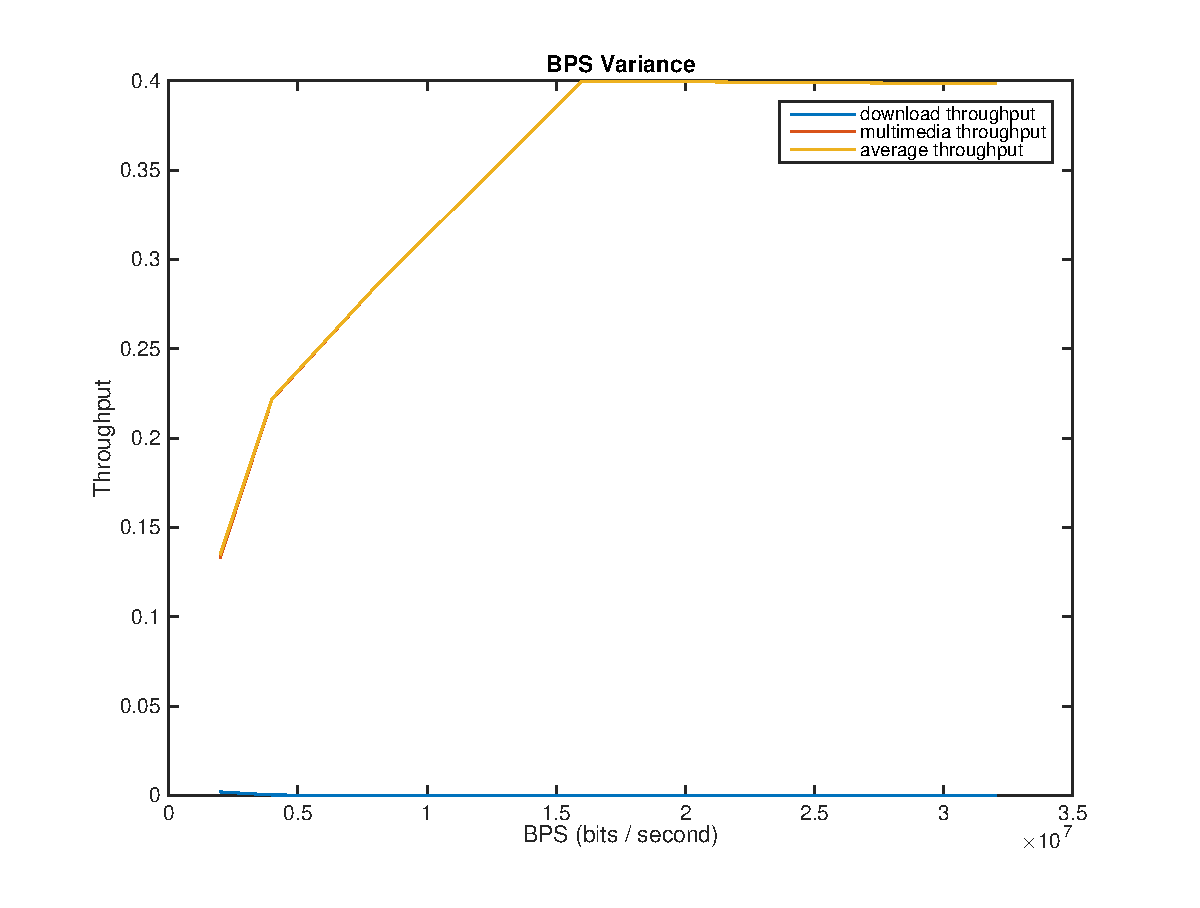
\includegraphics[scale=0.35]{../../src/fig-simulation_download_multimedia-bps-1_1_10_10_12000.eps} & 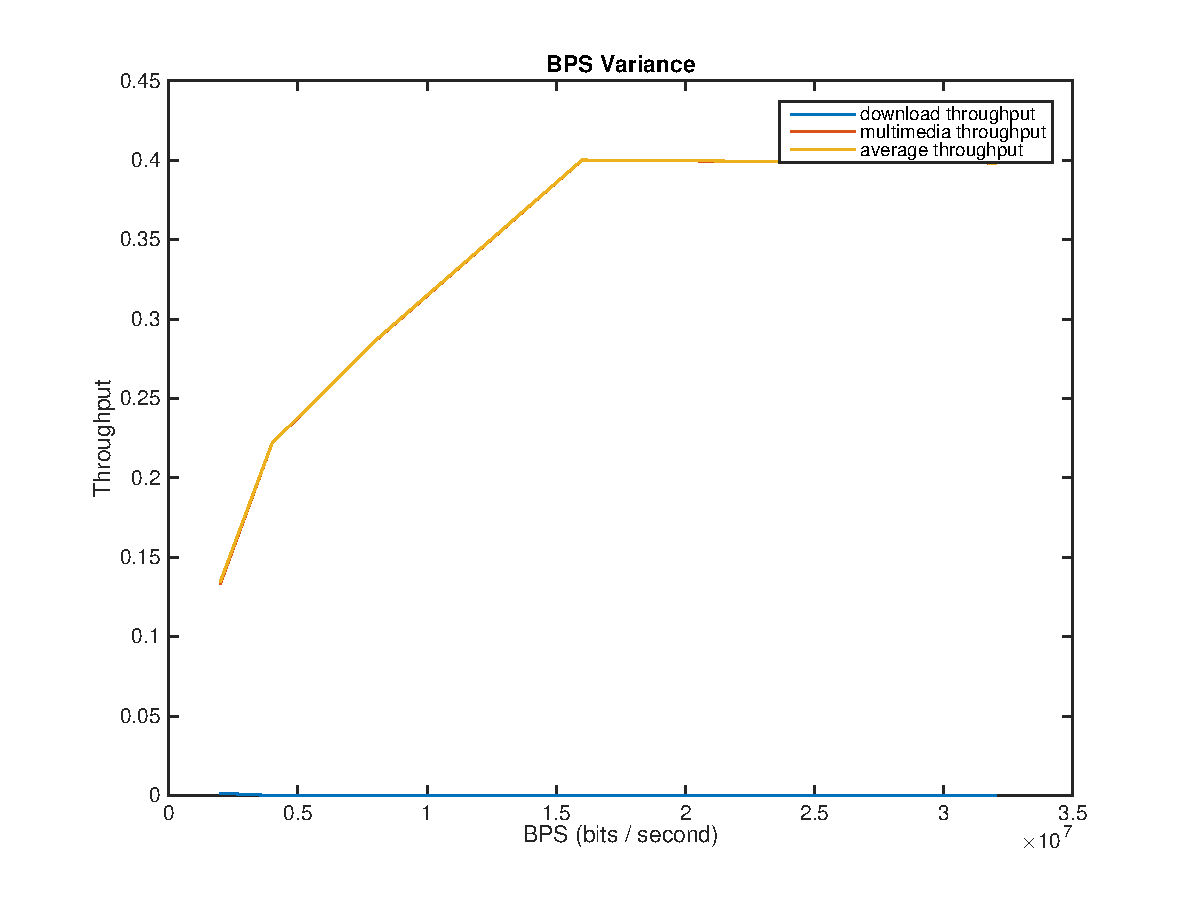
\includegraphics[scale=0.35]{../../src/fig-simulation_download_multimedia-bps-1_1_10_25_12000.eps} \\ 

% 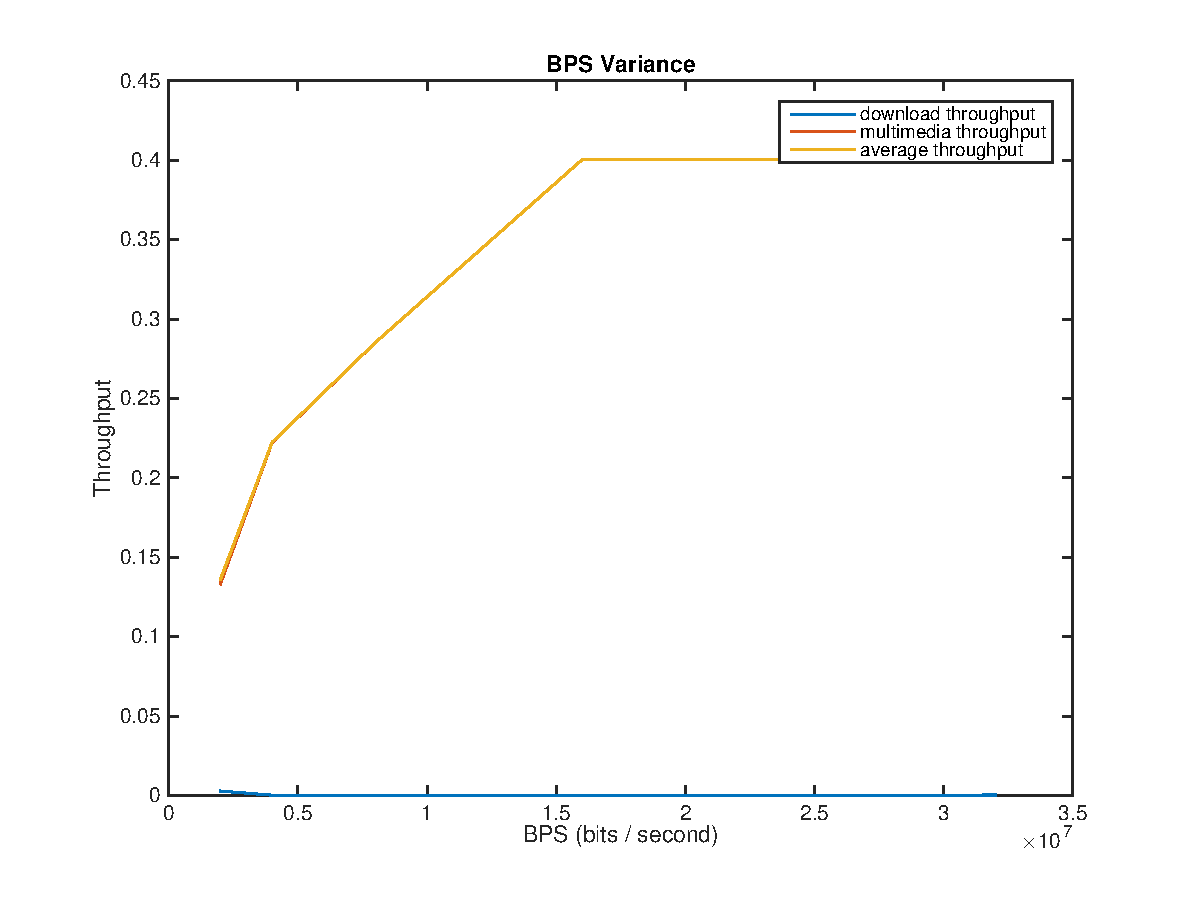
\includegraphics[scale=0.35]{../../src/fig-simulation_download_multimedia-bps-1_1_10_5_12000.eps} & 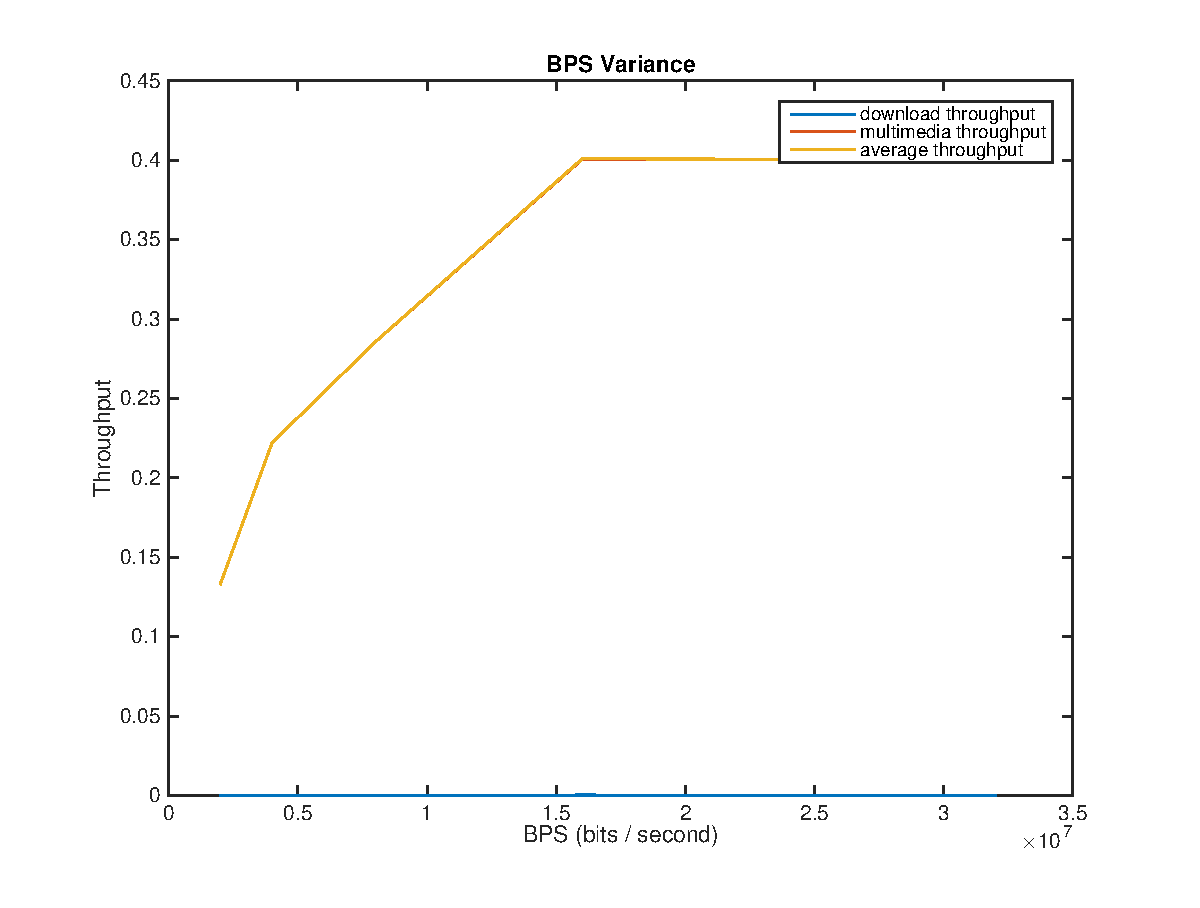
\includegraphics[scale=0.35]{../../src/fig-simulation_download_multimedia-bps-1_1_25_10_12000.eps} \\

% 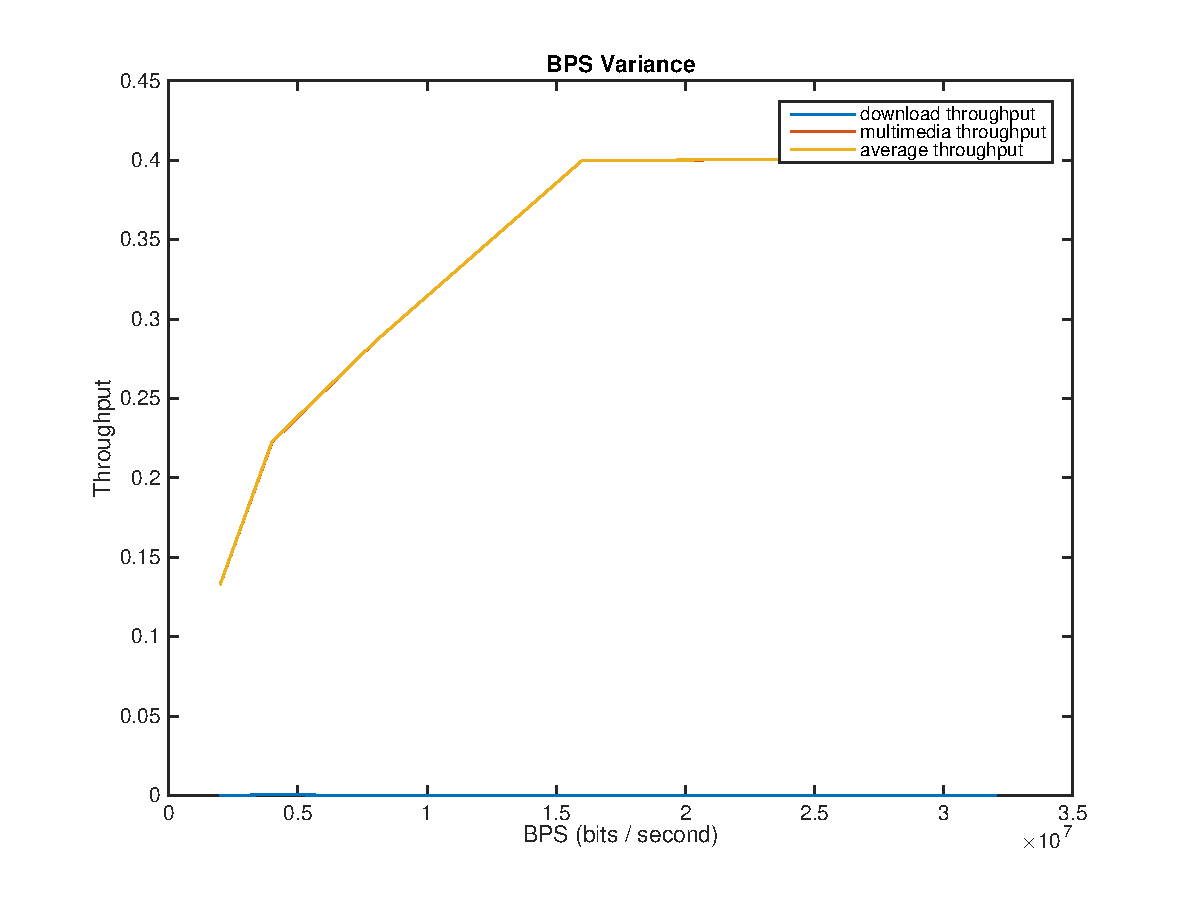
\includegraphics[scale=0.35]{../../src/fig-simulation_download_multimedia-bps-1_1_25_25_12000.eps} & 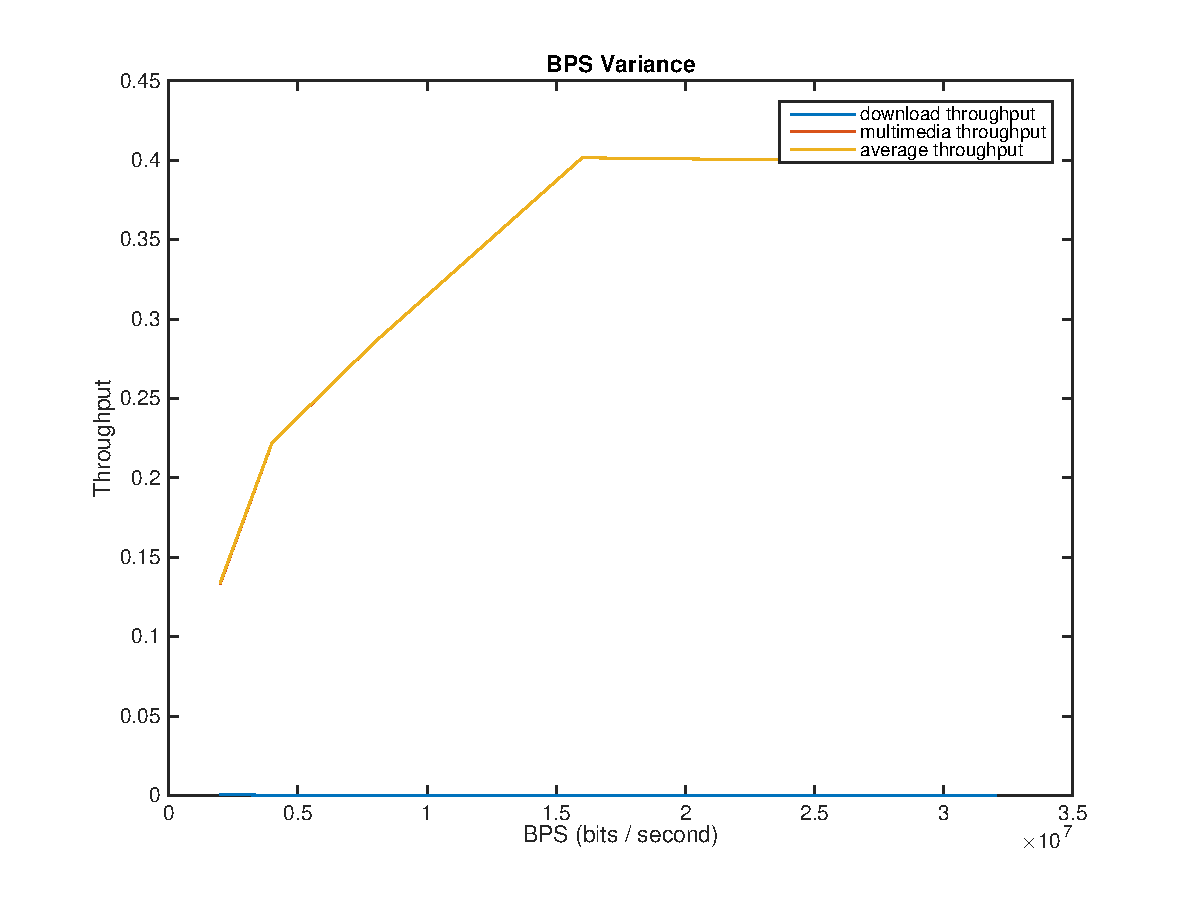
\includegraphics[scale=0.35]{../../src/fig-simulation_download_multimedia-bps-1_1_25_5_12000.eps} \\ 

% 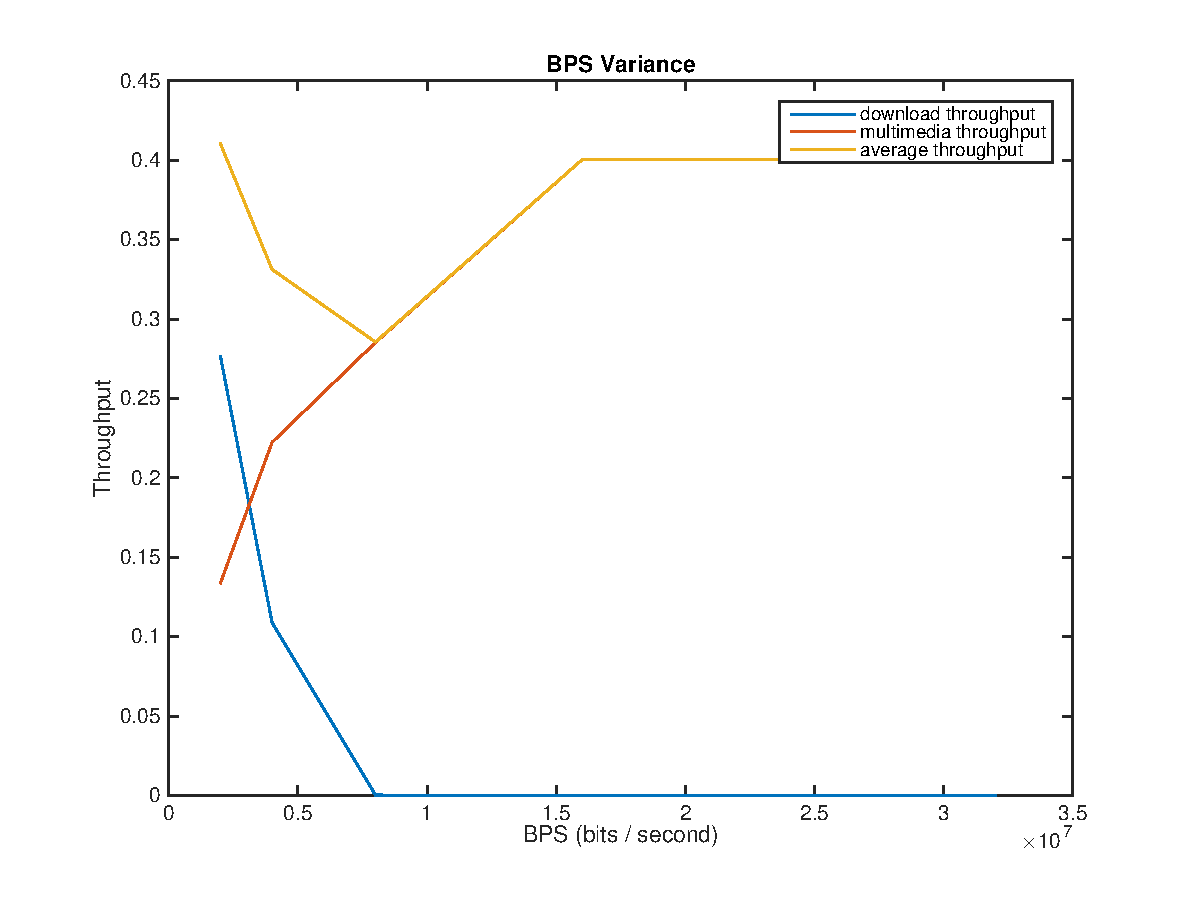
\includegraphics[scale=0.35]{../../src/fig-simulation_download_multimedia-bps-1_1_5_10_12000.eps} & 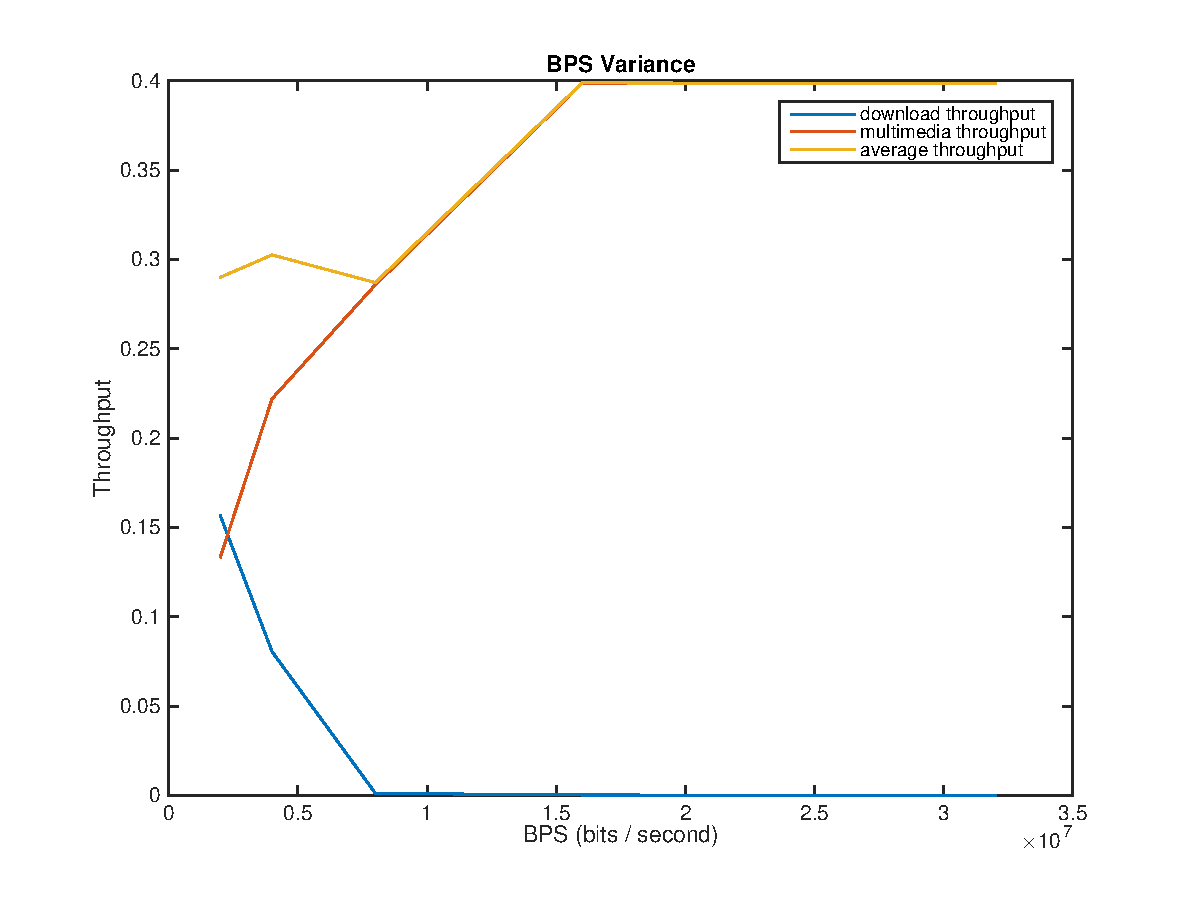
\includegraphics[scale=0.35]{../../src/fig-simulation_download_multimedia-bps-1_1_5_25_12000.eps}

% \end{tabular}
% \end{figure*}
\begin{figure*}
\begin{center}
\begin{tabular}{cc}
% 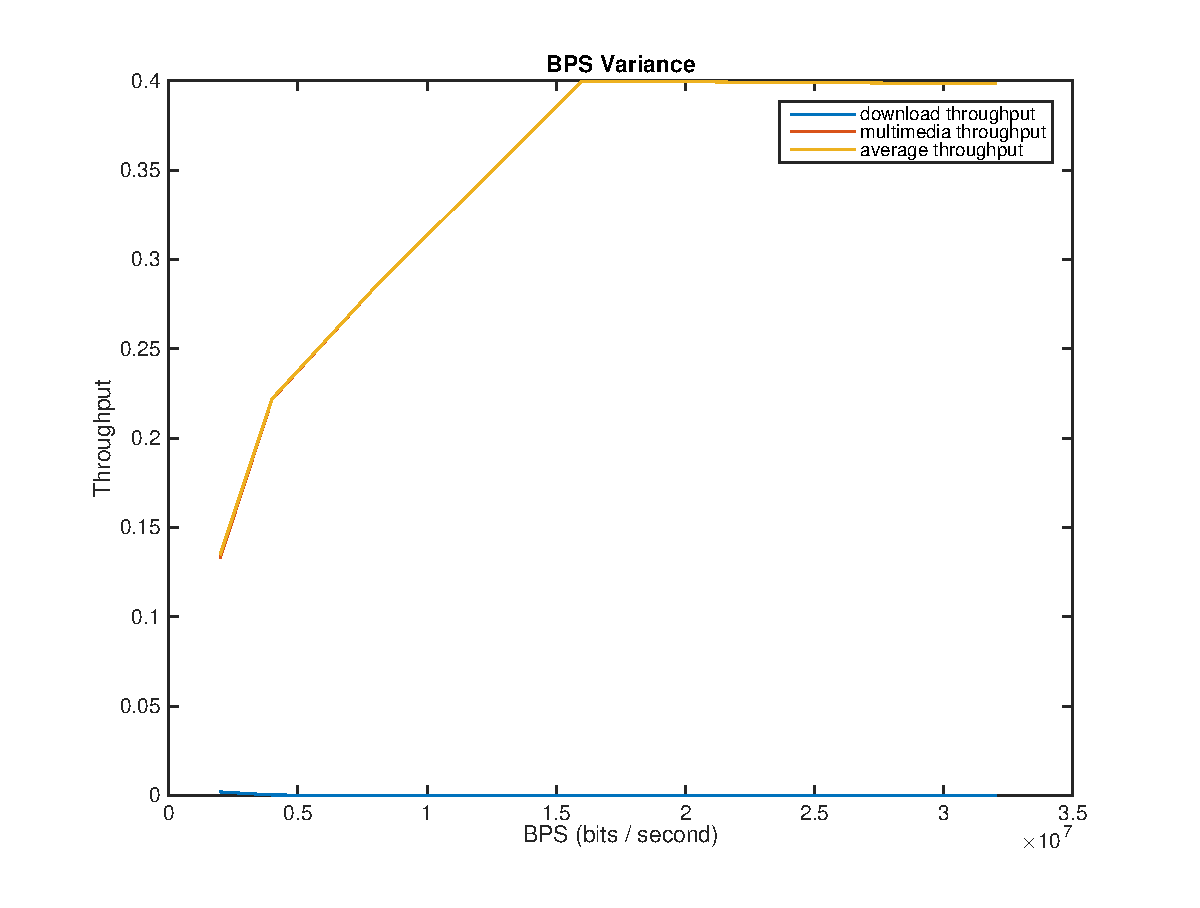
\includegraphics[scale=0.35]{../../src/fig-simulation_download_multimedia-bps-1_1_10_10_12000.eps} & 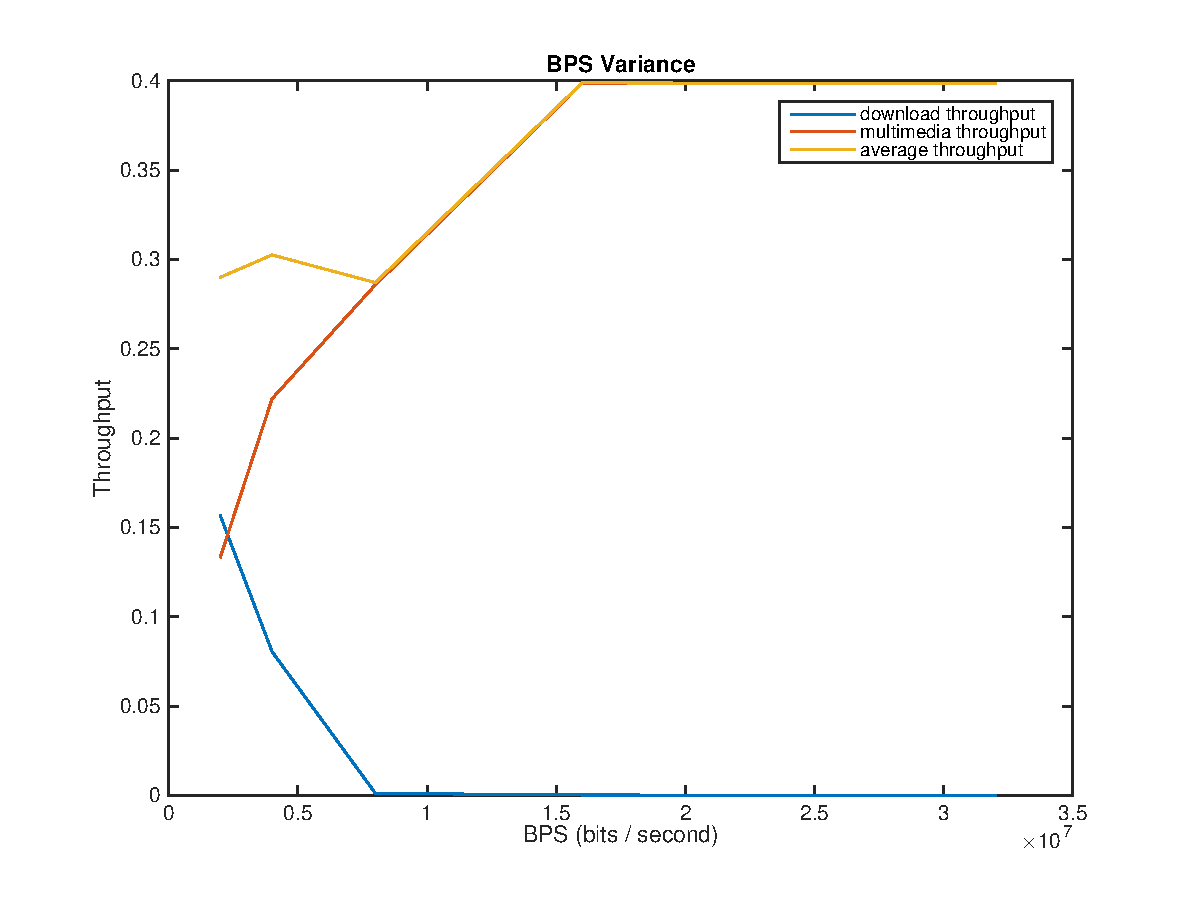
\includegraphics[scale=0.35]{../../src/fig-simulation_download_multimedia-bps-1_1_5_25_12000.eps} \\ 
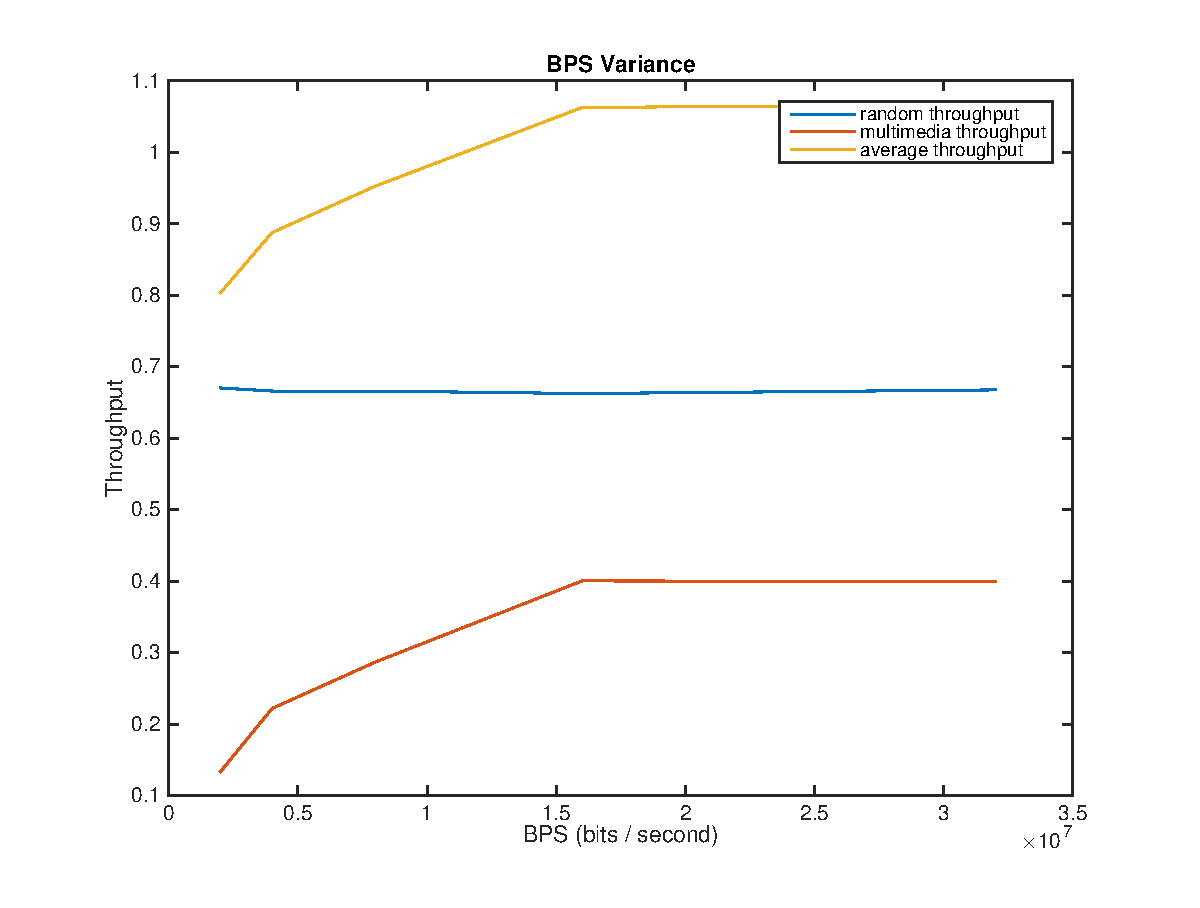
\includegraphics[scale=0.35]{../../src/fig-simulation_random_multimedia-bps-1_0_1_0_12000.eps} & 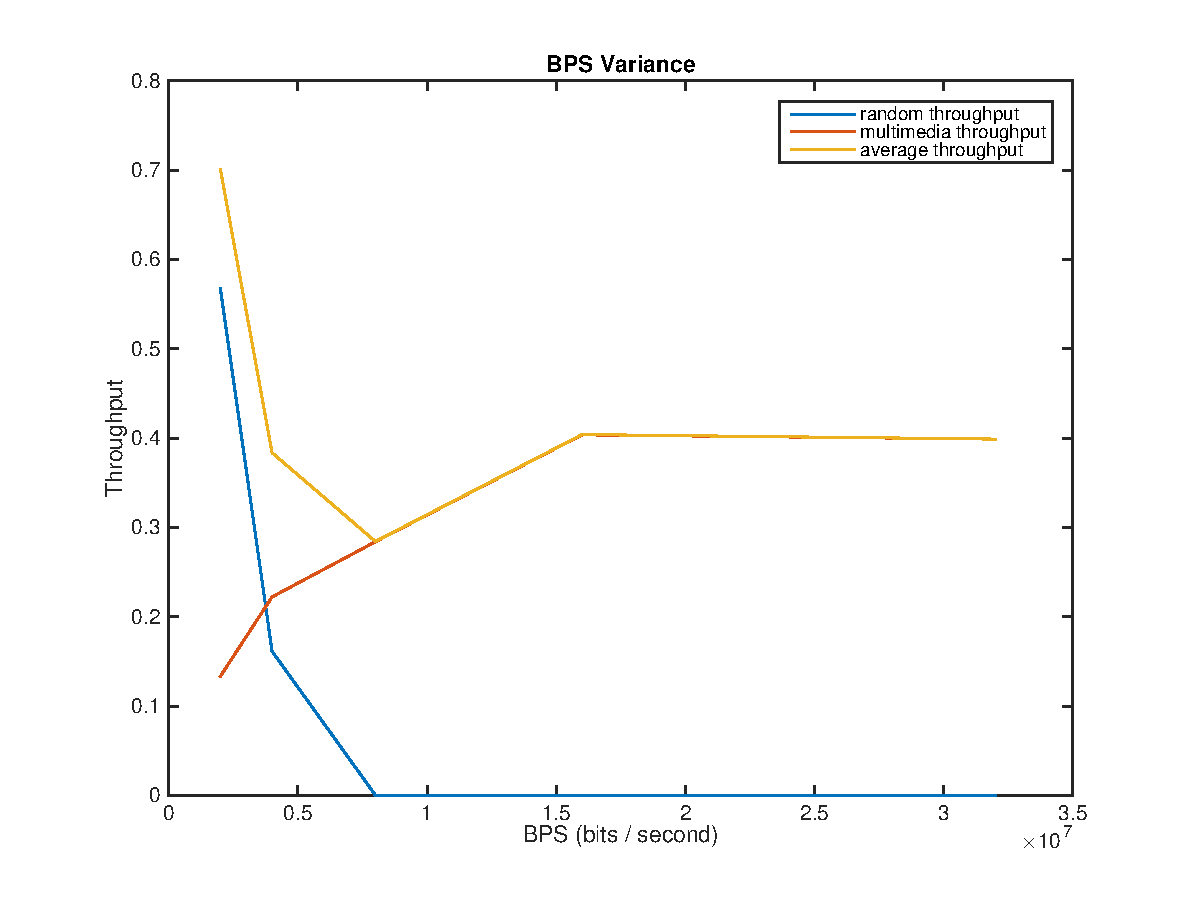
\includegraphics[scale=0.35]{../../src/fig-simulation_random_multimedia-bps-1_0_5_0_12000.eps}
\end{tabular}
\caption{The left figure shows the node and average throughput variance as a function of the multimedia node streaming BPS, compared to a random node with saturated traffic and packet sizes uniformly ranging from 1-5. The right figure shows the throughput in an identical scenario, except the random node packet size is always 1.}
\label{fig:randomstuff1}
\end{center}
\end{figure*}

%%% second
% \begin{figure*}
% \begin{tabular}{cc}

% 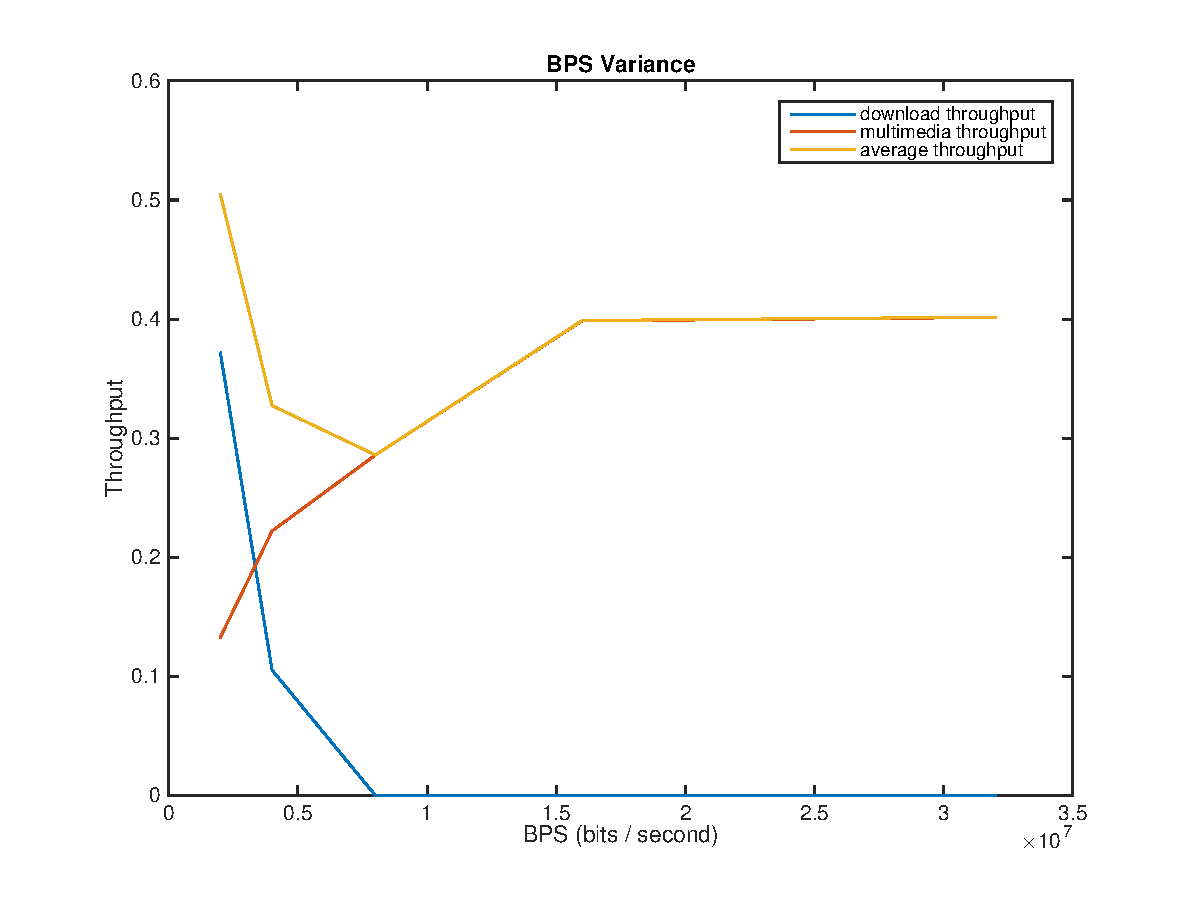
\includegraphics[scale=0.35]{../../src/fig-simulation_download_multimedia-bps-1_1_5_5_12000.eps} & 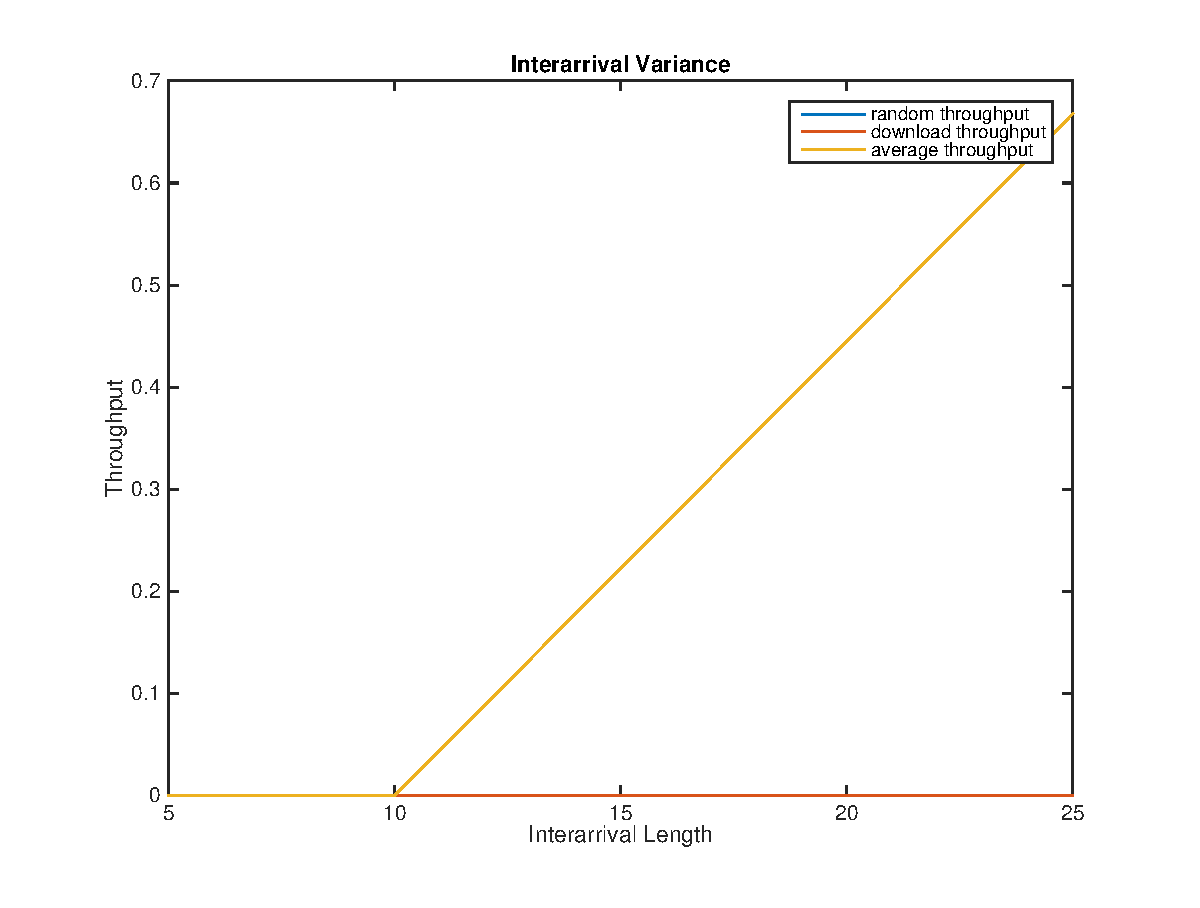
\includegraphics[scale=0.35]{../../src/fig-simulation_random_download-interarival-1_0_1_0_1_1_25.eps} \\
% 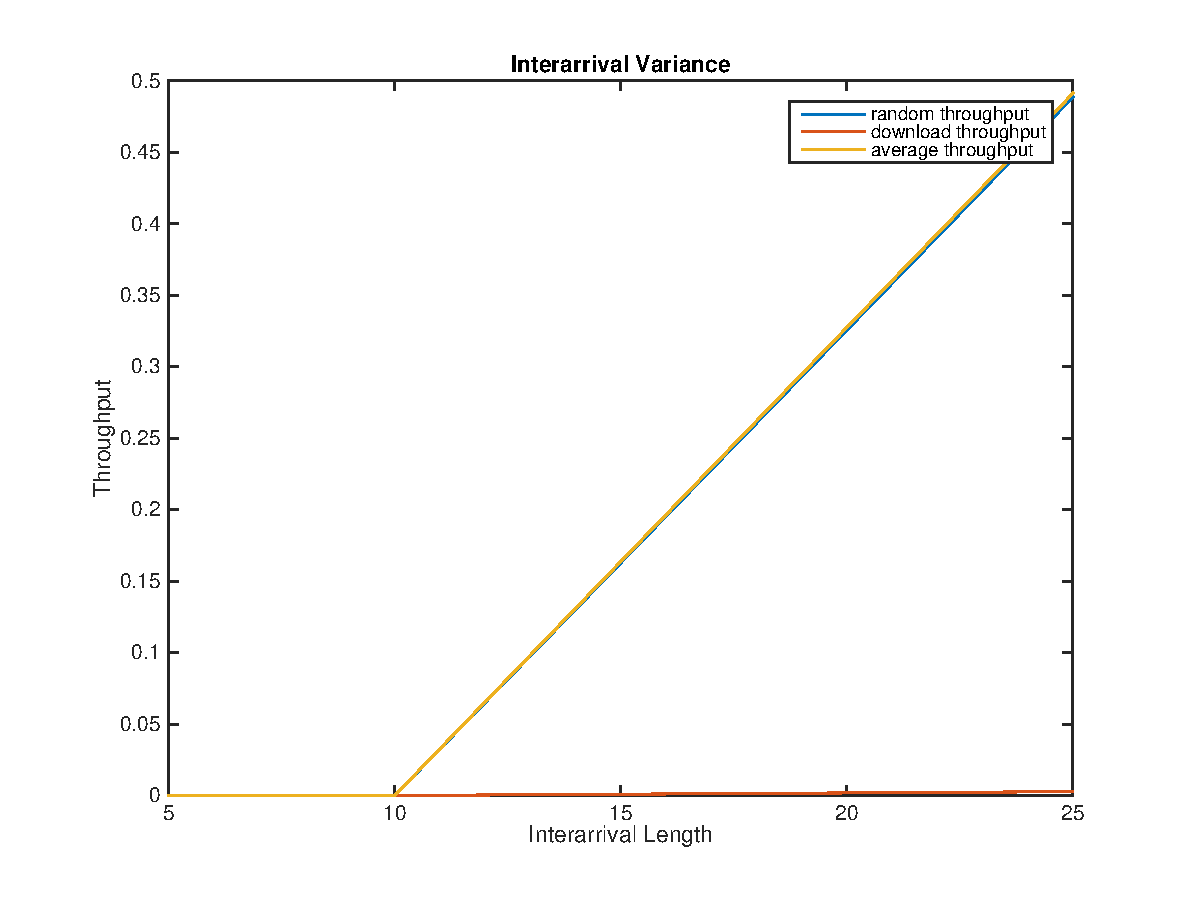
\includegraphics[scale=0.35]{../../src/fig-simulation_random_download-interarival-1_0_5_0_1_1_25.eps} & 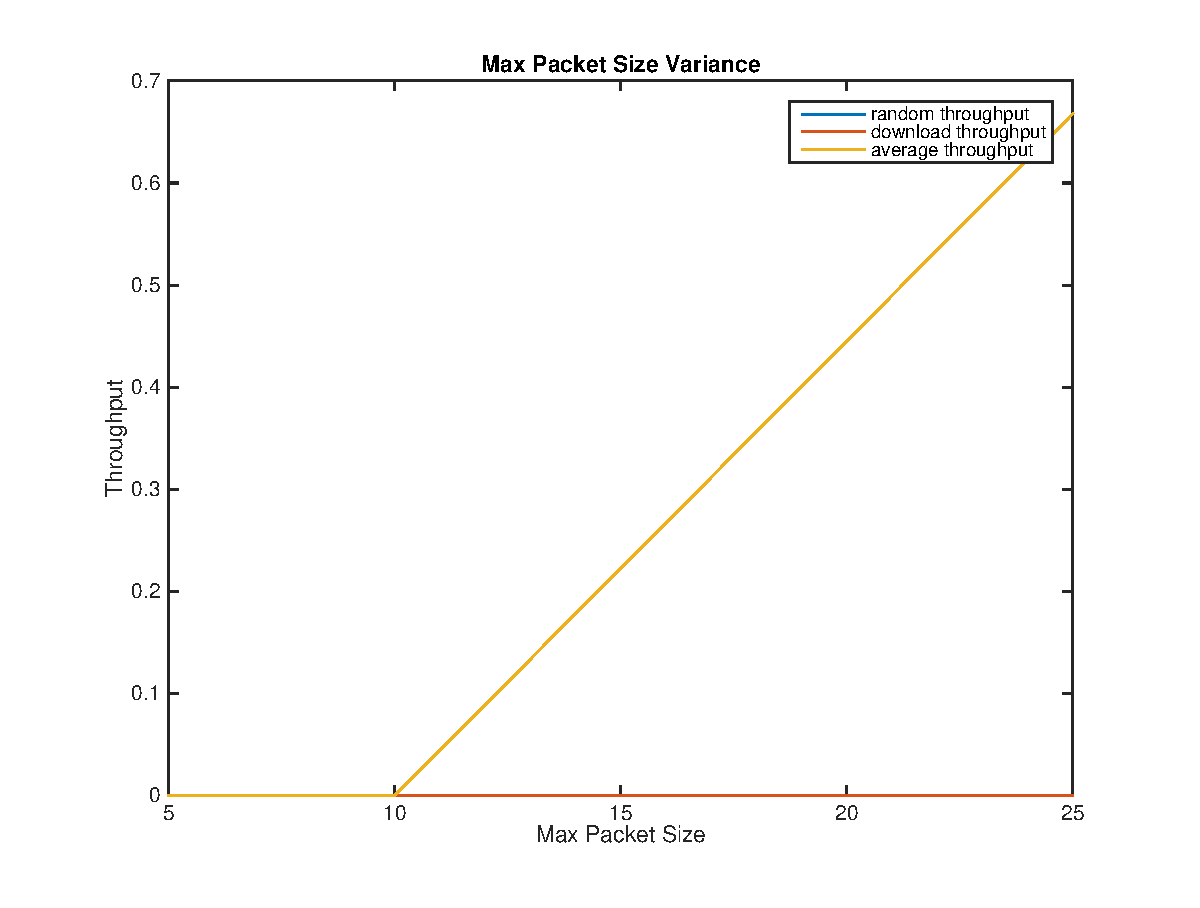
\includegraphics[scale=0.35]{../../src/fig-simulation_random_download-maxpackets-1_0_1_0_1_1_25.eps} \\
% 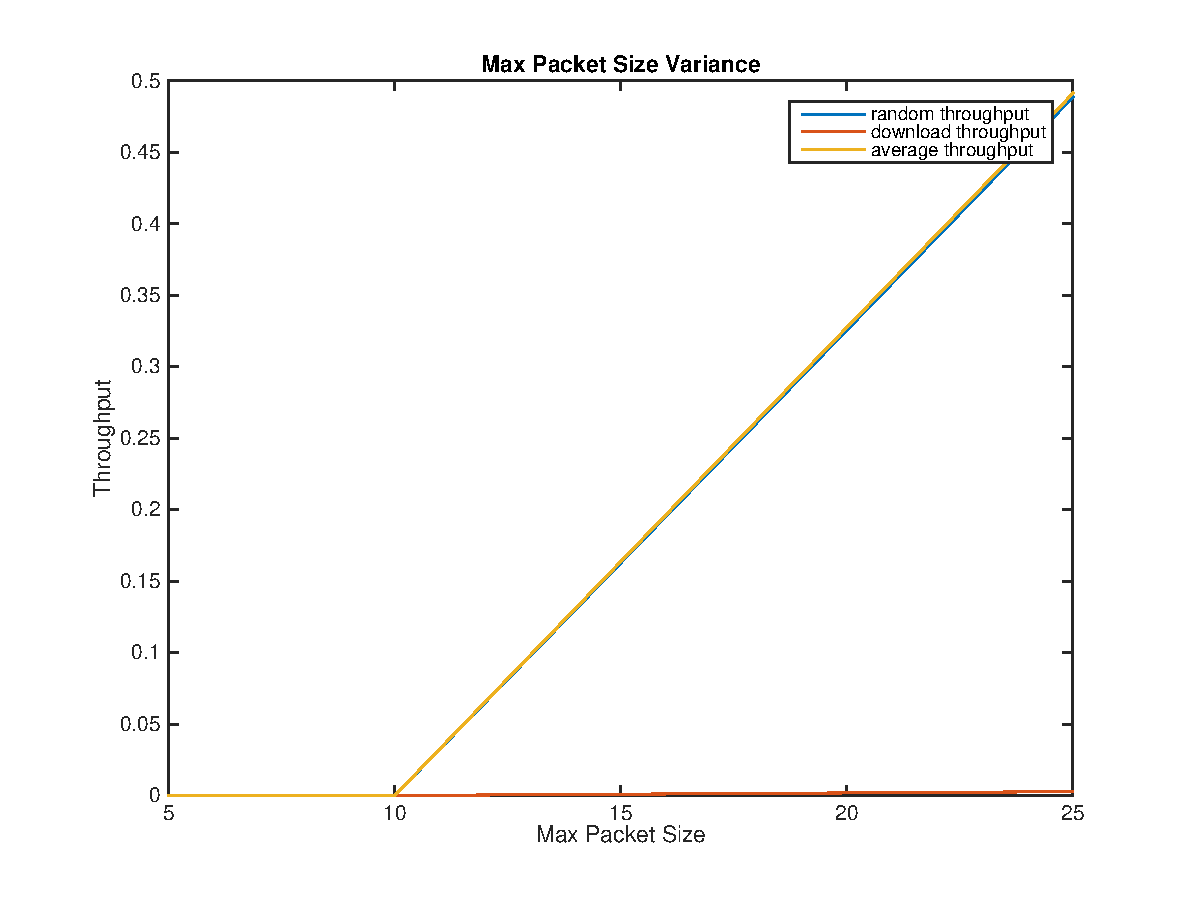
\includegraphics[scale=0.35]{../../src/fig-simulation_random_download-maxpackets-1_0_5_0_1_1_25.eps} & 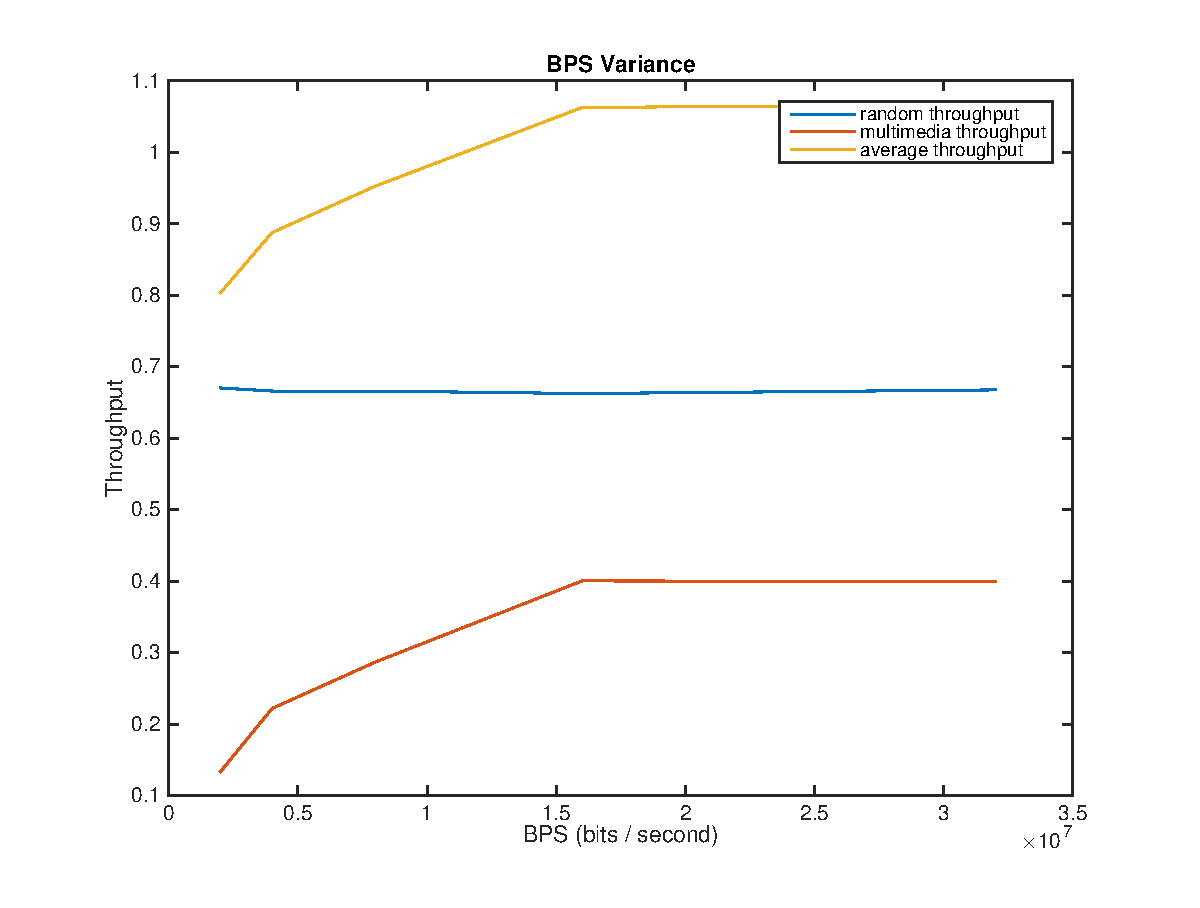
\includegraphics[scale=0.35]{../../src/fig-simulation_random_multimedia-bps-1_0_1_0_12000.eps} \\
% 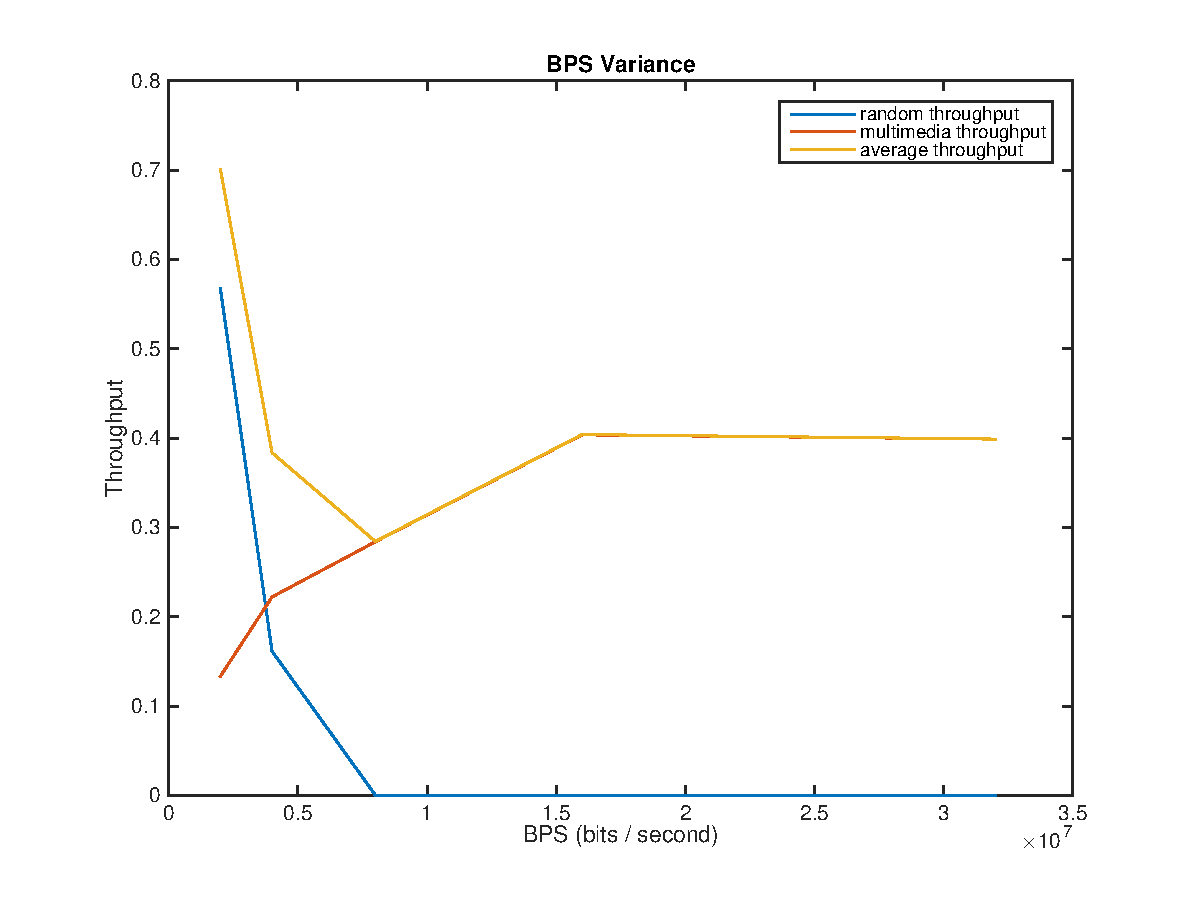
\includegraphics[scale=0.35]{../../src/fig-simulation_random_multimedia-bps-1_0_5_0_12000.eps} & 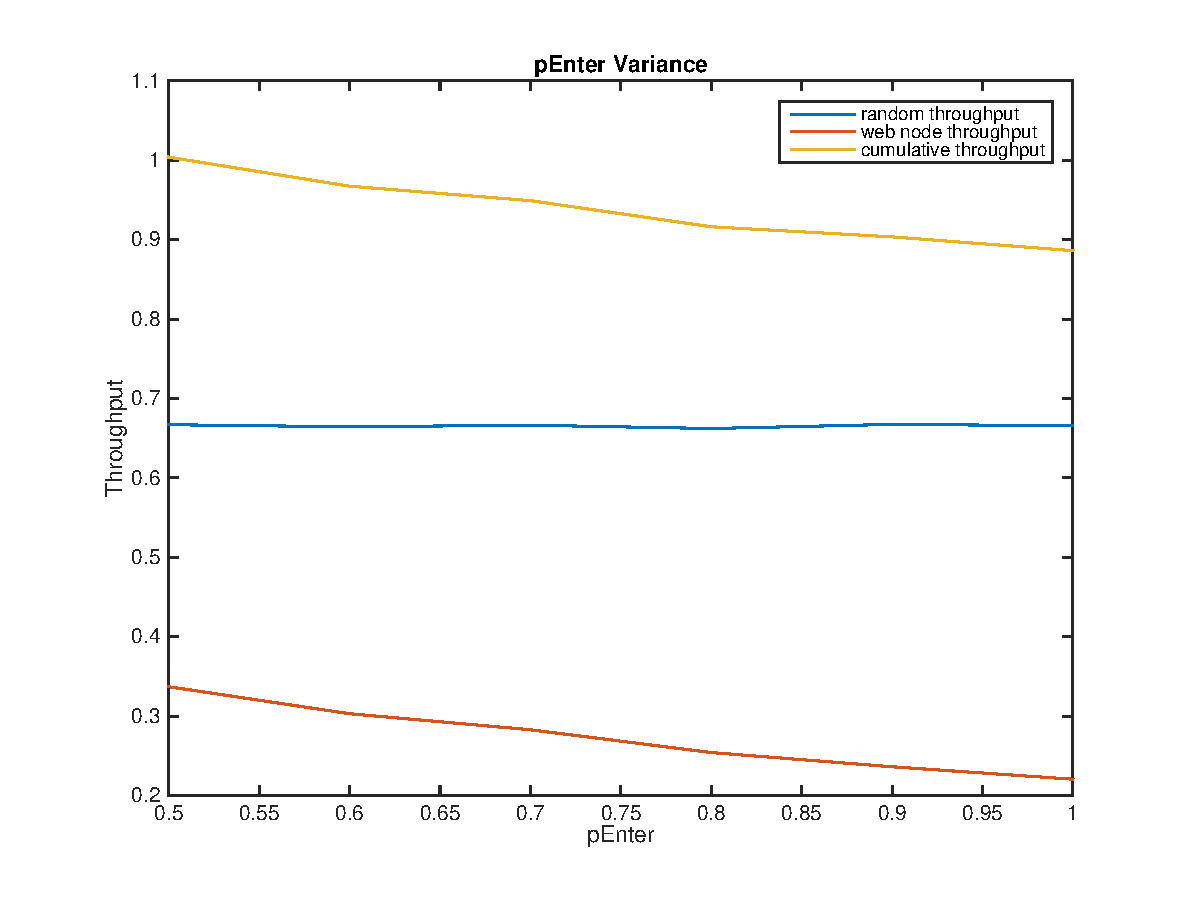
\includegraphics[scale=0.35]{../../src/fig-simulation_random_web-penter-1_0_1_0_1_1_5.eps}

% \end{tabular}
% \end{figure*}
\begin{figure*}
\begin{center}
\begin{tabular}{cc}

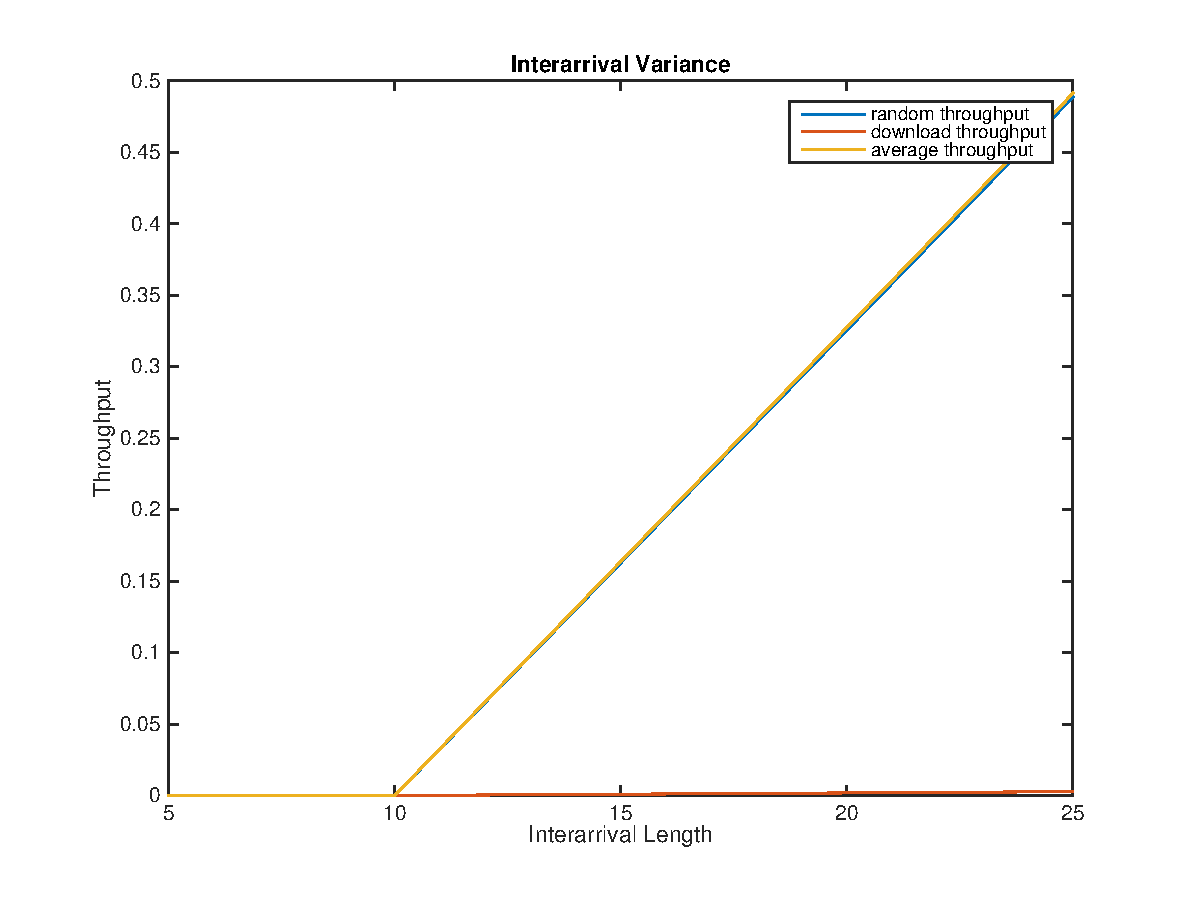
\includegraphics[scale=0.35]{../../src/fig-simulation_random_download-interarival-1_0_5_0_1_1_25.eps} & 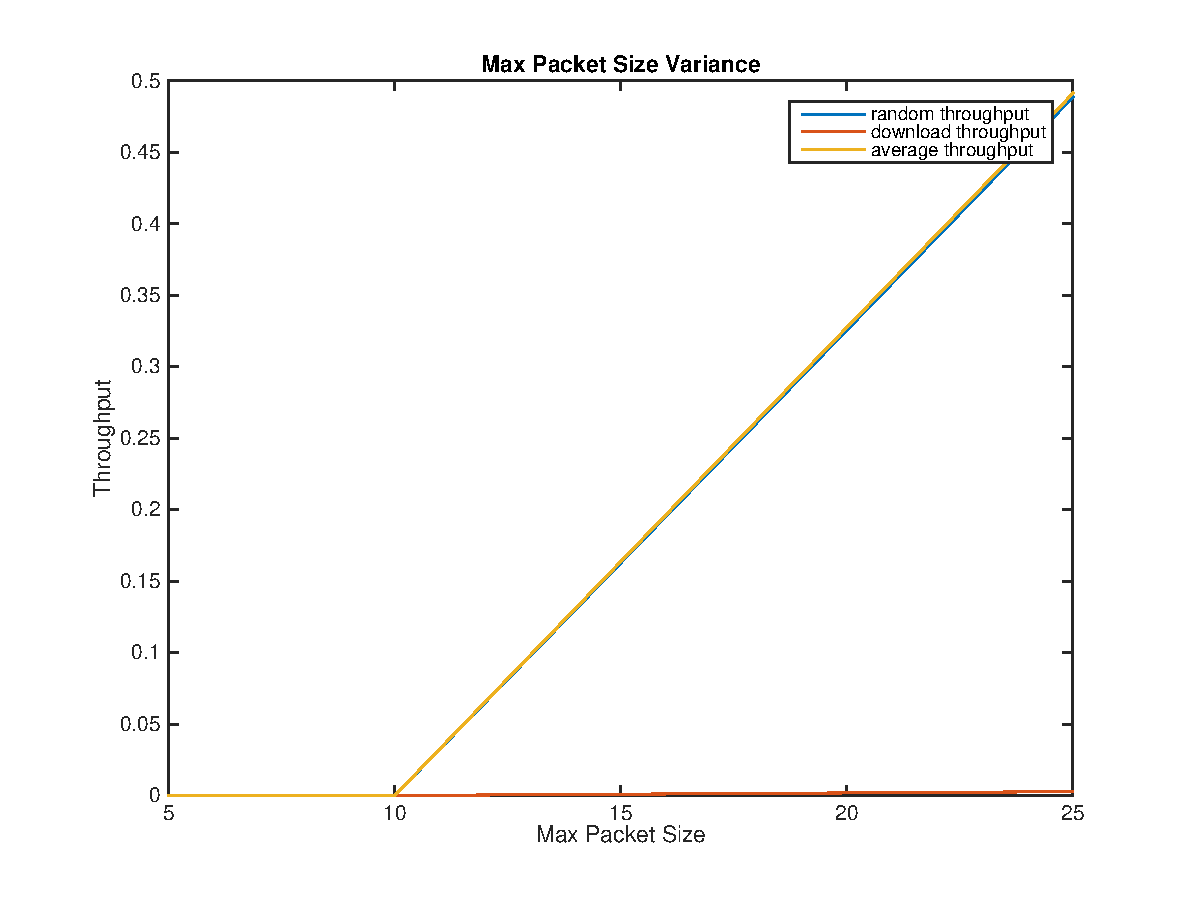
\includegraphics[scale=0.35]{../../src/fig-simulation_random_download-maxpackets-1_0_5_0_1_1_25.eps} \\
% 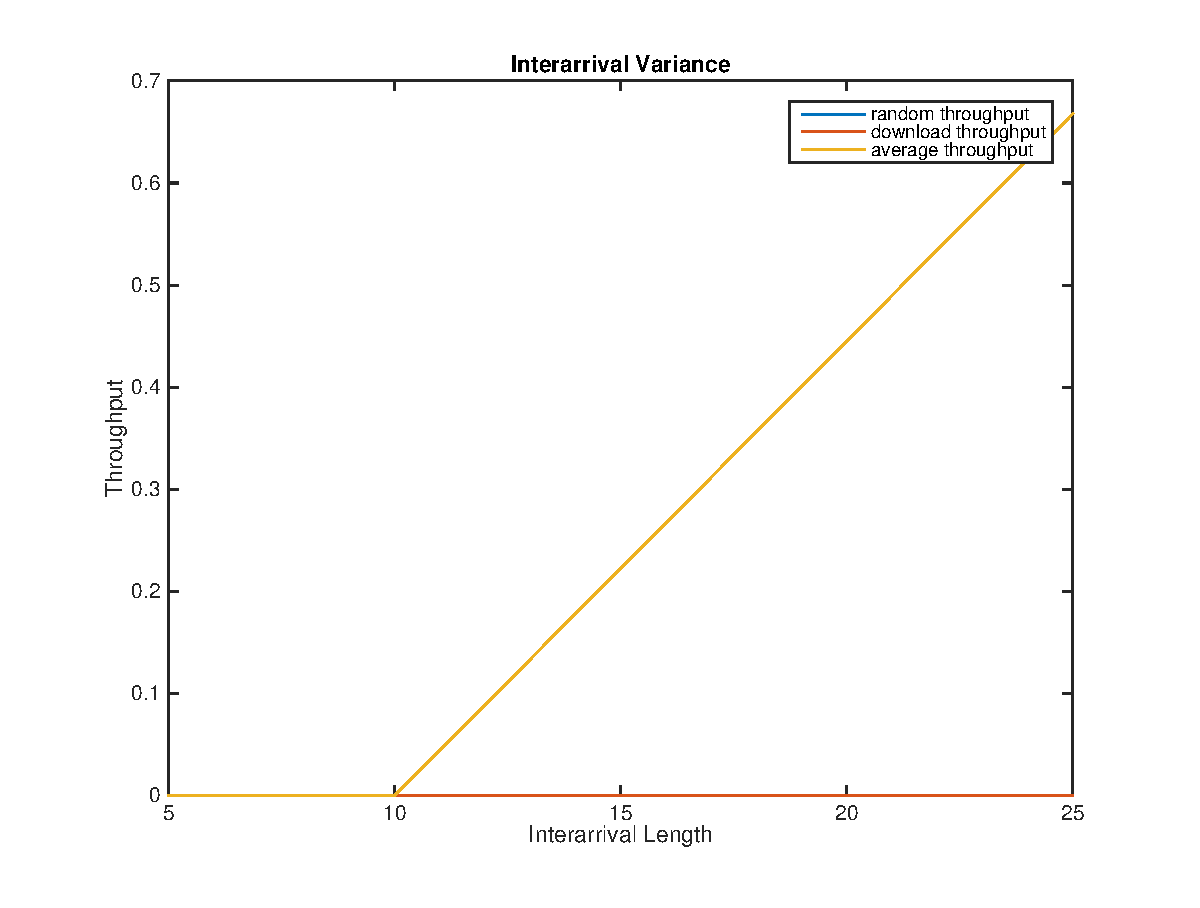
\includegraphics[scale=0.35]{../../src/fig-simulation_random_download-interarival-1_0_1_0_1_1_25.eps} & 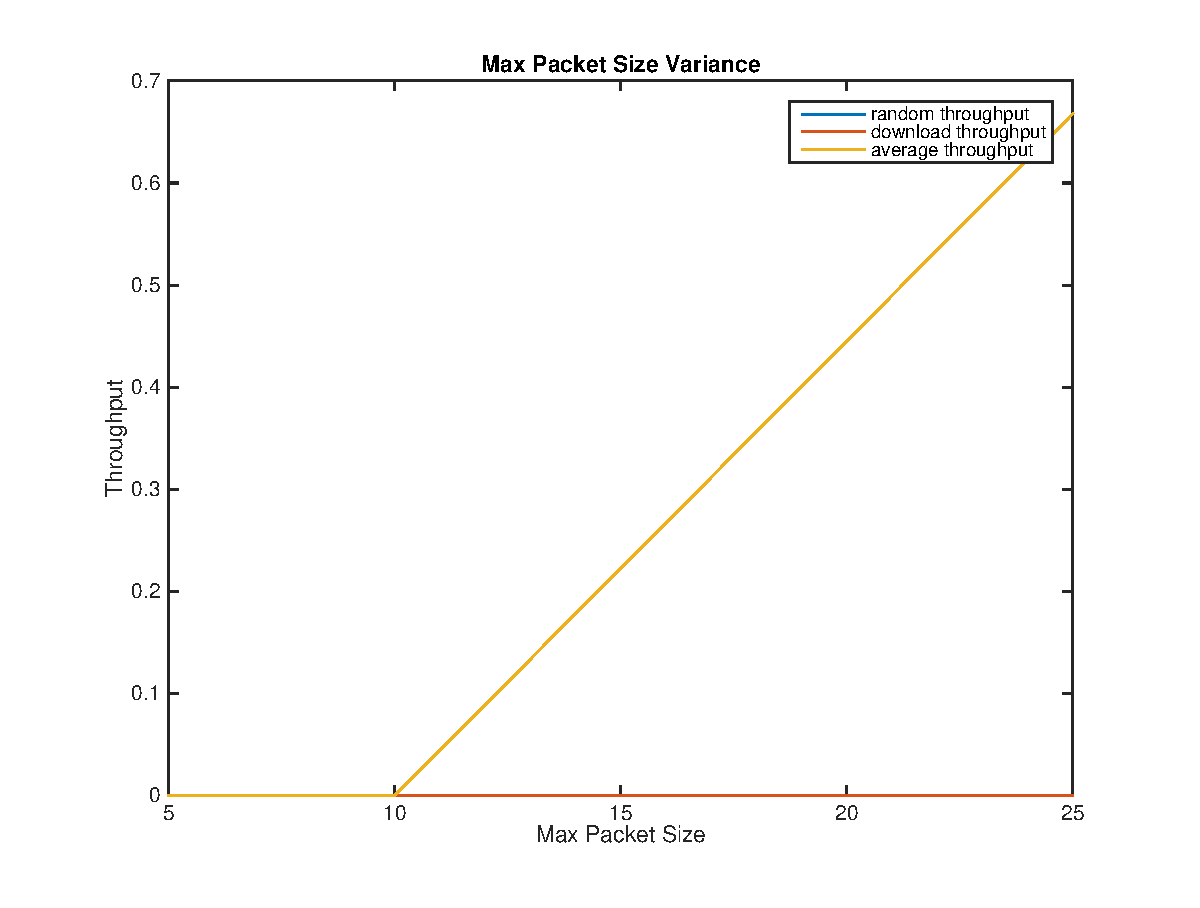
\includegraphics[scale=0.35]{../../src/fig-simulation_random_download-maxpackets-1_0_1_0_1_1_25.eps} \\
\end{tabular}
\caption{The left figure shows the node and average throughput variance as a function of the file download interarrival length, compared to a random node with saturated traffic and packet sizes of length 1. The right figure shows the throughput in an identical scenario, except the random node has packet sizes uniformly ranging from 1-5.}
\label{fig:randomstuff2}
\end{center}
\end{figure*}

%%% third
% \begin{figure*}
% \begin{tabular}{cc}

% 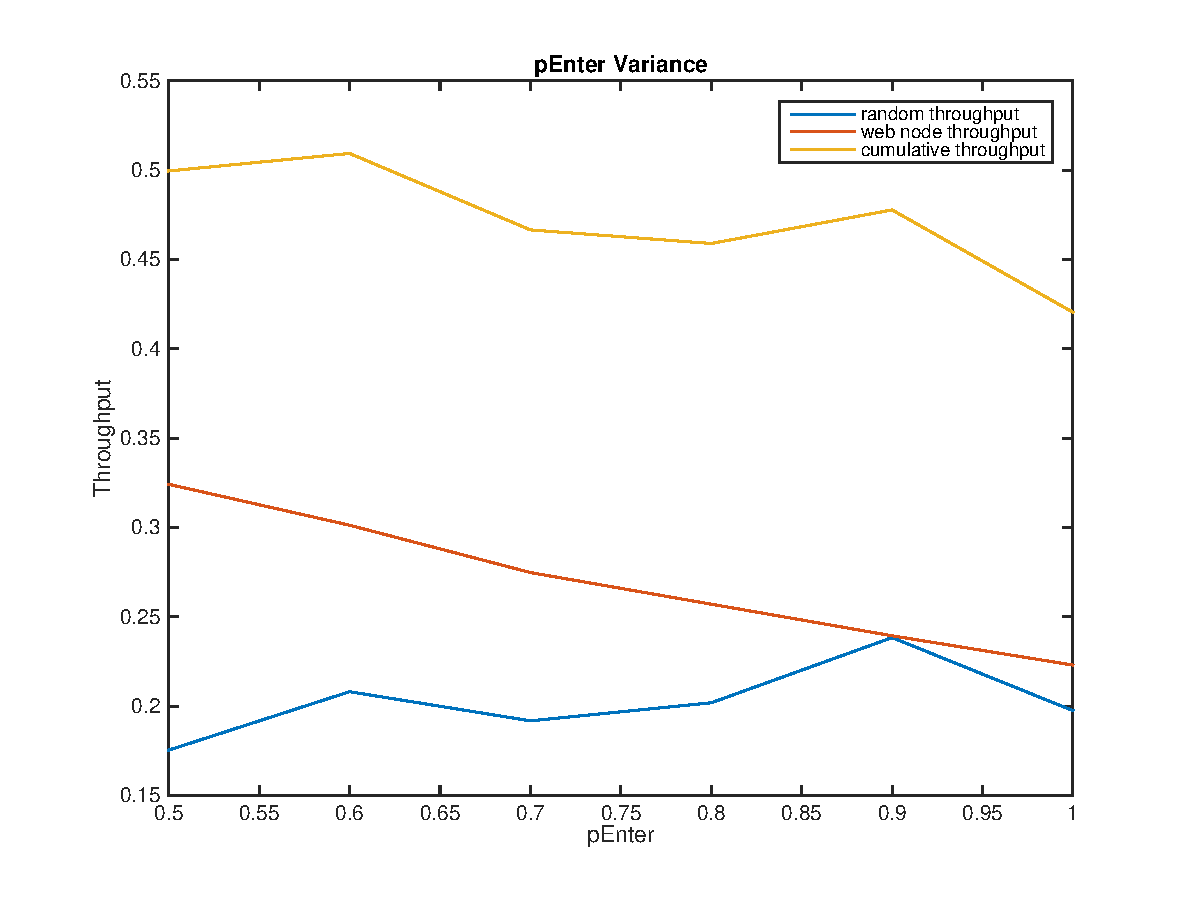
\includegraphics[scale=0.35]{../../src/fig-simulation_random_web-penter-1_0_5_0_1_1_5.eps} & 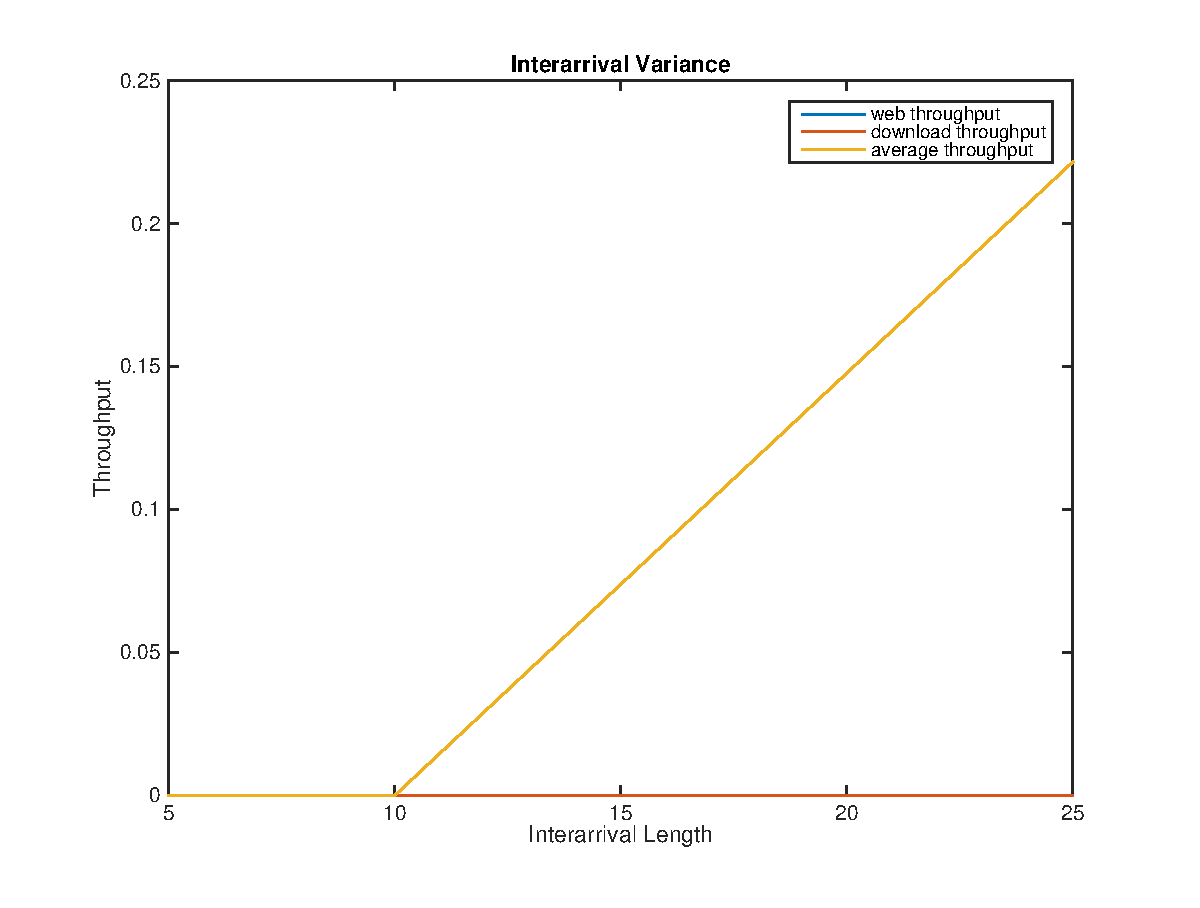
\includegraphics[scale=0.35]{../../src/fig-simulation_web_download-interarival-1_1_1_5_1_1_25.eps} \\
% \includegraphics[scale=0.35]{../../src/fig-simulation_web_download-interarival-1_5_000000e-01_1_5_1_1_25.eps} & 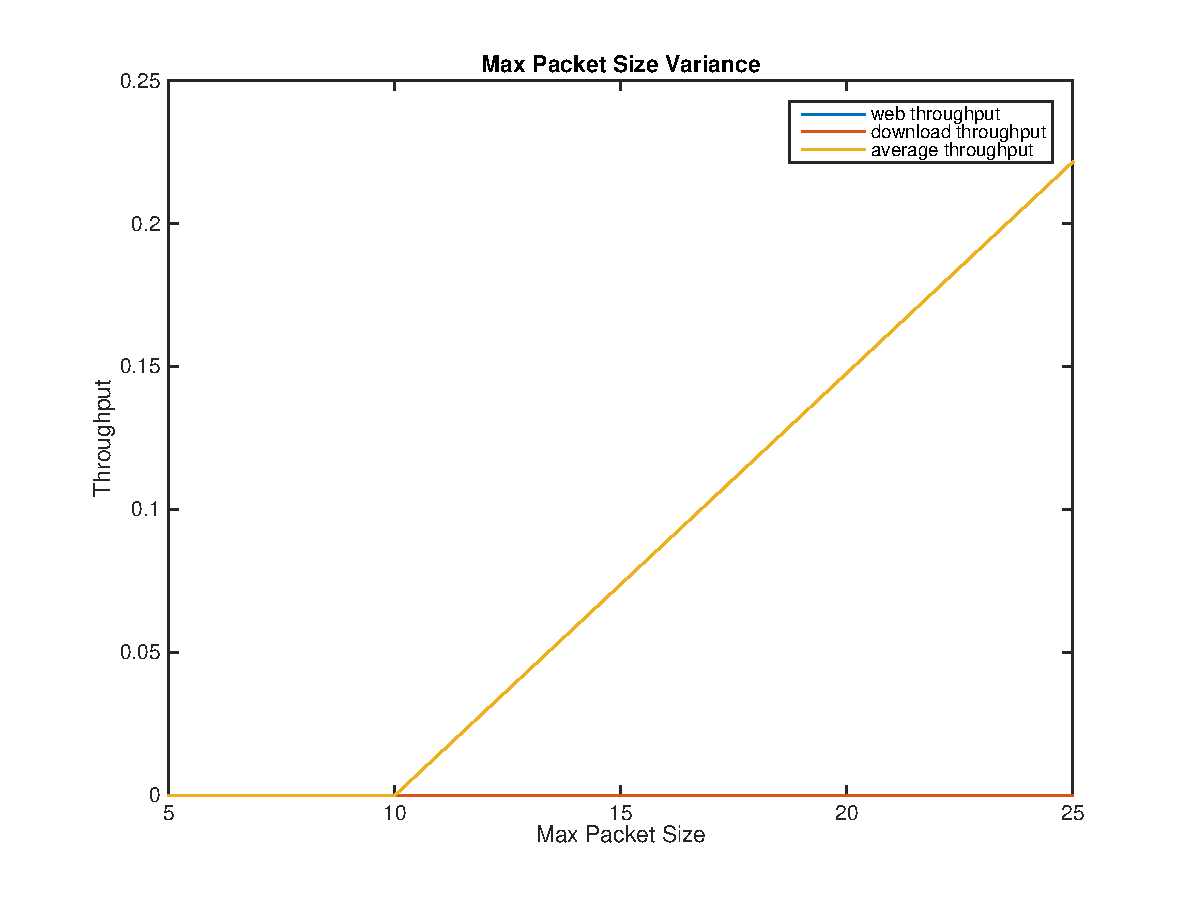
\includegraphics[scale=0.35]{../../src/fig-simulation_web_download-maxpackets-1_1_1_5_1_1_25.eps} \\
% \includegraphics[scale=0.35]{../../src/fig-simulation_web_download-maxpackets-1_5_000000e-01_1_5_1_1_25.eps} & 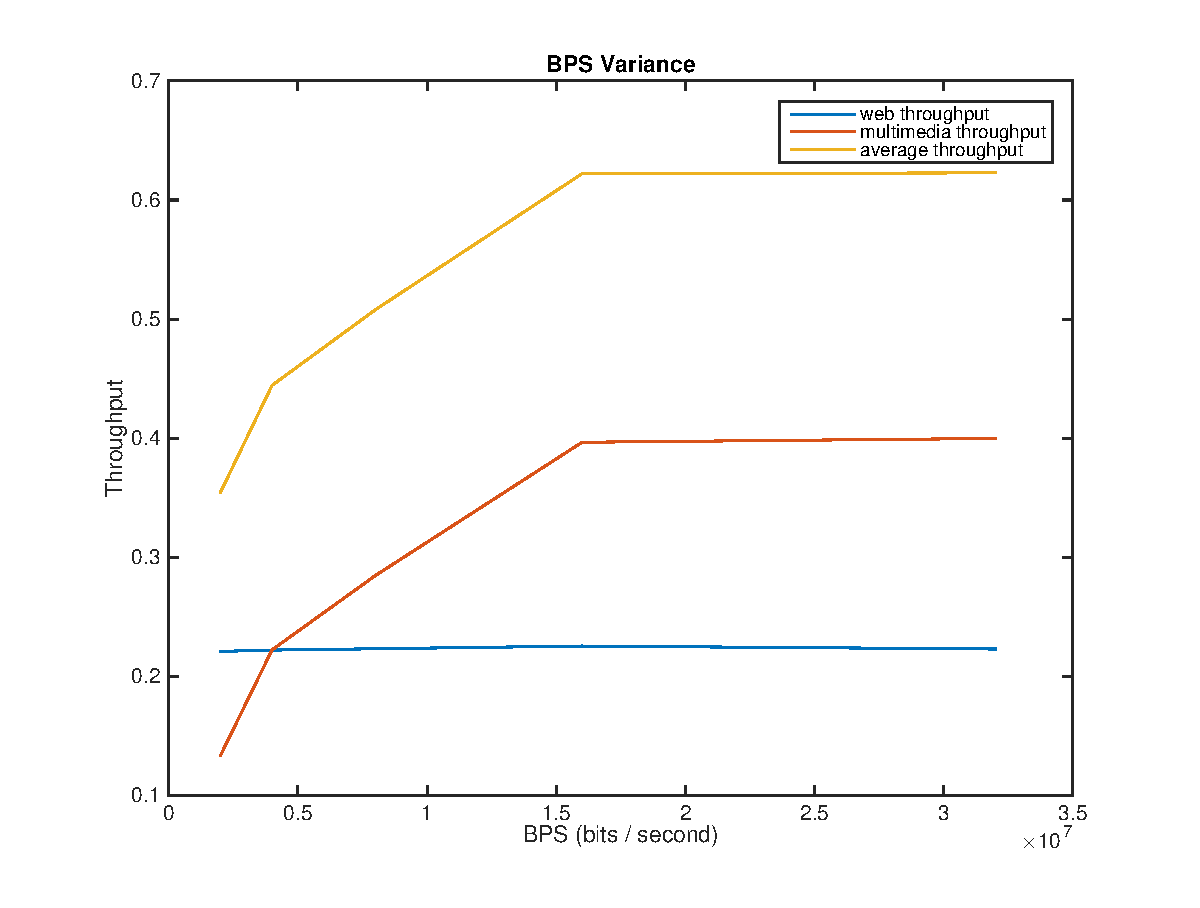
\includegraphics[scale=0.35]{../../src/fig-simulation_web_multimedia-bps-1_1_1_5_12000.eps} \\

% \multicolumn{2}{c}{\includegraphics[scale=0.35]{../../src/fig-simulation_web_multimedia-bps-1_5_000000e-01_1_5_12000.eps}}

% \end{tabular}
% \end{figure*}

\begin{figure*}
\begin{center}
\begin{tabular}{cc}

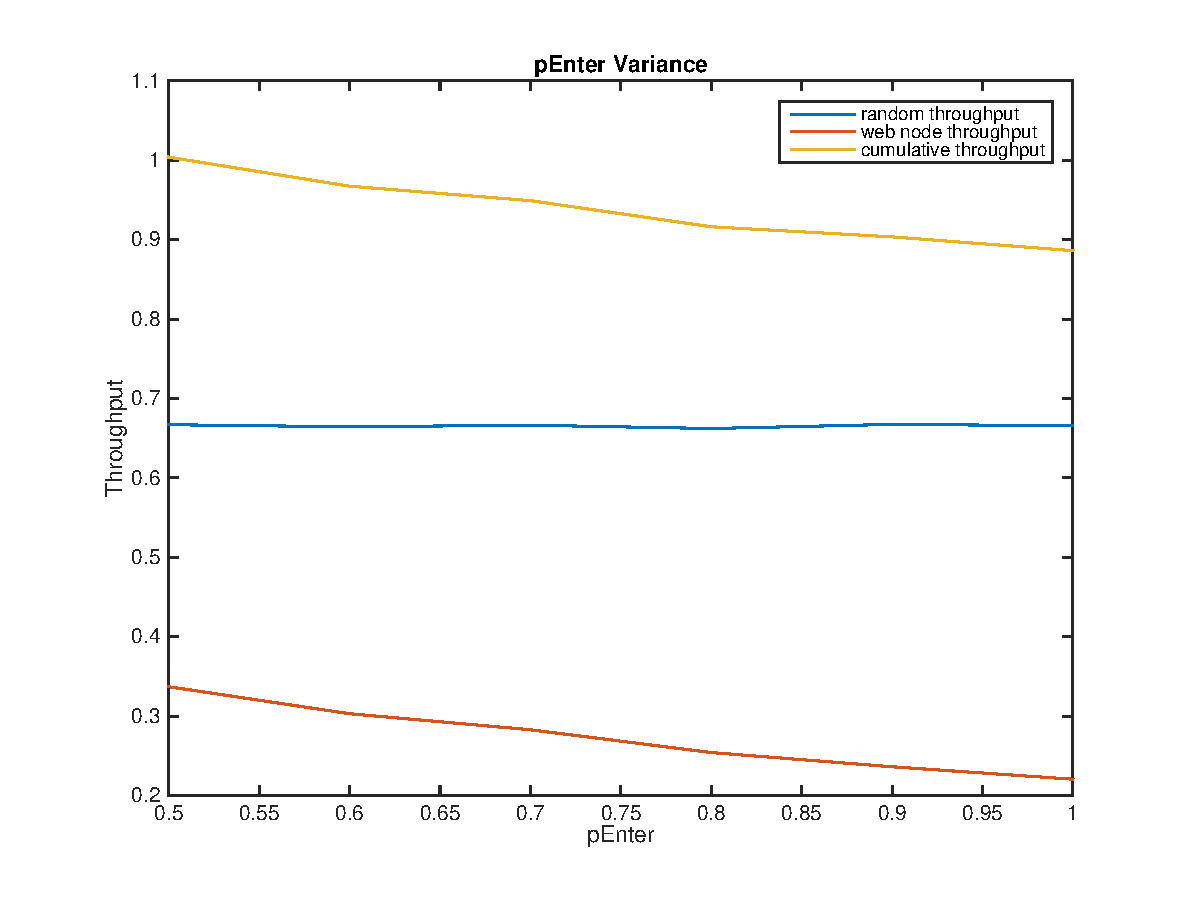
\includegraphics[scale=0.35]{../../src/fig-simulation_random_web-penter-1_0_1_0_1_1_5.eps} & 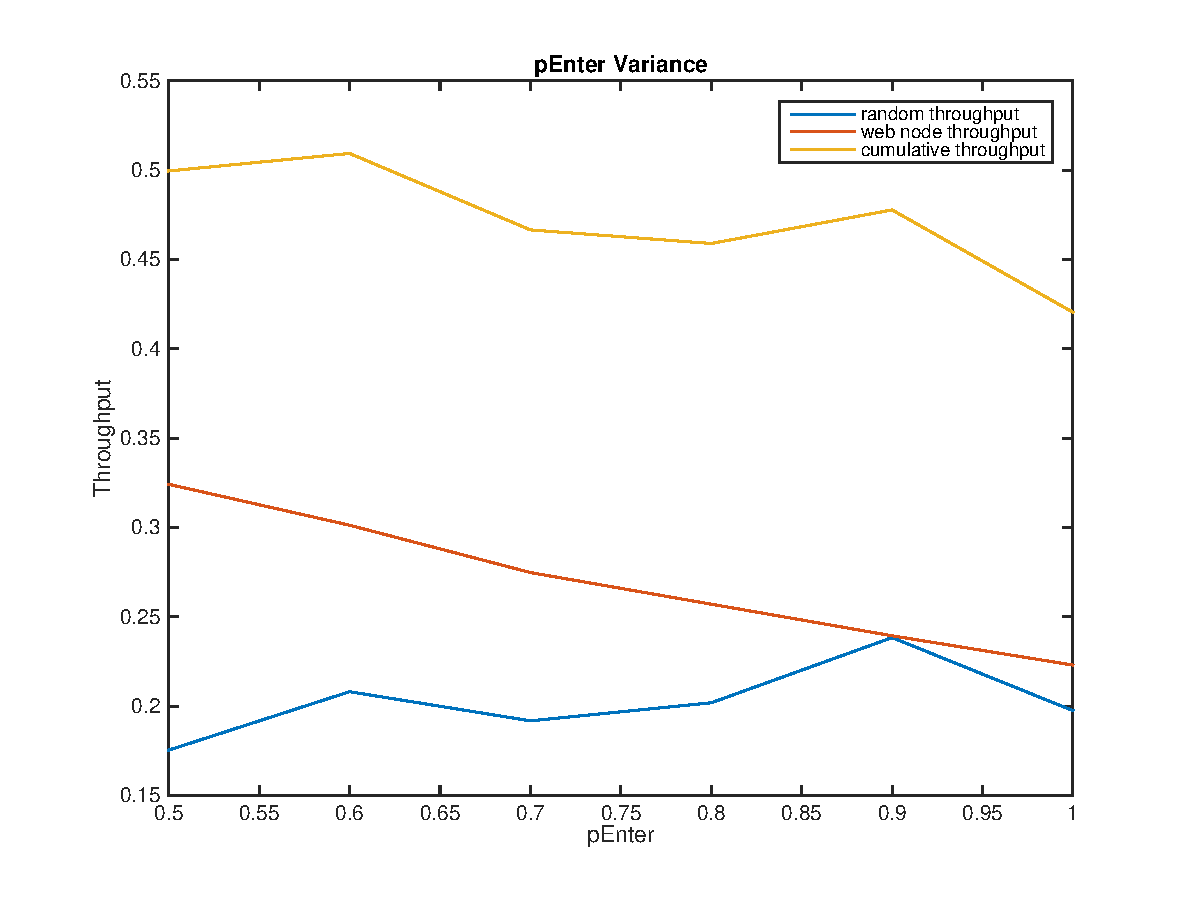
\includegraphics[scale=0.35]{../../src/fig-simulation_random_web-penter-1_0_5_0_1_1_5.eps} \\
\end{tabular}
\caption{The left figure shows the node and average throughput variance as a function of the interarrival probability, compared to a random node with saturated traffic with packet sizes of length 1. The right figure shows the throughput in an identical scenario, except the random node has packet sizes uniformly ranging from 1-5.}
\label{fig:randomstuff3}
\end{center}
\end{figure*}